
%(BEGIN_QUESTION)
% Copyright 2006, Tony R. Kuphaldt, released under the Creative Commons Attribution License (v 1.0)
% This means you may do almost anything with this work of mine, so long as you give me proper credit

A {\it single-phase bridge rectifier} circuit is made of four diodes, arranged like this:

$$\includegraphics[width=15.5cm]{i01437x01.eps}$$

Trace the directions of current through all four diodes, and determine the polarity of DC voltage across the motor terminals.

\vskip 10pt

A {\it three-phase bridge rectifier} circuit is made of six diodes, arranged like this:

$$\includegraphics[width=15.5cm]{i01437x02.eps}$$

Once again, trace the directions of current through all six diodes, and determine the polarity of DC voltage across the motor terminals.

\underbar{file i01437}
%(END_QUESTION)





%(BEGIN_ANSWER)

$$\includegraphics[width=15.5cm]{i01437x04.eps}$$

$$\includegraphics[width=15.5cm]{i01437x03.eps}$$
 
%(END_ANSWER)





%(BEGIN_NOTES)

%INDEX% Electronics review: bridge rectifiers

%(END_NOTES)


